\documentclass[11pt]{article}

%####### DON'T CHANGE MARGIN SETTINGS ###########
\newcommand{\keywordfont}{\textsc}
\newcommand{\keyword}[1]{%
  \marginpar{\raggedright\small\keywordfont{#1}}}
\reversemarginpar
\usepackage[a4paper, top=2.5cm, bottom=2.5cm, outer=2cm, inner=3.3cm, marginparwidth=72pt, heightrounded]{geometry}
%#################################

 \usepackage{amsmath}
\usepackage{amssymb}
\usepackage{hyperref}
\usepackage{graphicx}
\usepackage{microtype}

\begin{document}

\Large
\begin{center}
\textbf{MA3K7 Big Mini Project - Rubric}
\\
Timothy Yap (2161367)
\end{center}
\normalsize

%--------------------------------------------------------------------------------------------------
% Problem 3: A pub game

% On a table in the Varsity pub, a number of empty pint glasses are placed in a circular
% arrangement. Each glass holds exactly a pint of liquid and the glasses are identical.
% Maths students Ali and Beth play the following game.

% • Ali takes half a pint of water in a small glass (from the bar) and distributes the
% water amongst the pint glasses in any way they wish.

% • Beth then takes two adjacent pint glasses on the table, empties them (say, out the
% window) and puts them back into the circular arrangement.

% Ali wants to make one of the glasses overflow, and Beth wants to prevent this.

% Investigate.

%--------------------------------------------------------------------------------------------------

\section{Entry} %----------------------------------------------------------------------------------

We will be investigating Problem 3: A pub game. \keyword{Problem Description} This two-player game begins with some empty glasses in a circular arrangement, with each glass holding up to a pint of liquid. Our two players have different objectives. One is trying to make at least one glass overflow, and the other is trying to prevent this.

In our problem description, we have Ali and Beth playing our game, but we \keyword{Introduce} will introduce \textit{Player A}, who represents Ali, the person trying to make a glass overflow with water. Similarly, we introduce \textit{Player B}, who represents Beth, the person trying to stop Player A. We will also formally state that a \textit{turn} is one full complete action. For Player A, their turn is distributing their half pint of water fully. As for Player B, their turn is to empty two adjacent pint glasses. We will also use glass and cups interchangeably.

From an initial reading of our problem, we know \keyword{I know} the following:
\begin{itemize}
    \item  Player A and Player B alternate turns doing their respective action.
    \item For Player A to win, a glass must overflow. There has to be strictly more than one pint of water in one glass.
    \item For Player B to win, they must prevent any cup from having more than one pint of water. In theory, they would have to play forever to win but we will say that if they have a strategy that prevents Player A from overfilling a glass, they win. 
\end{itemize}

There are a few assumptions that we will state \keyword{Assumptions} before investigating our problem. Firstly, as in most idealise game theory scenarios, we assume that all players are rational and will act in their best interest, which is to win. Therefore Players A and B will not be impacted by any human factors and are acting as robots. Cold and calculative. Another assumption is that there will be $n$ number of glasses and that will remain the same throughout the game. Lastly, we assume Player A goes first as Player B would have nothing to remove if they went first.

Clarifying \keyword{Clarification} the problem, we have the glasses placed in a `circular' arrangement. We take this to be as shown in Figure 1 below. We may also use the linear representation to save space or when writing in table format. This is shown in Figure 2. We will just assume that the glasses labelled 1 and $n$ are adjacent to each other.

\begin{figure}[h]
    \centering
    \begin{minipage}{0.5\textwidth}
        \centering
        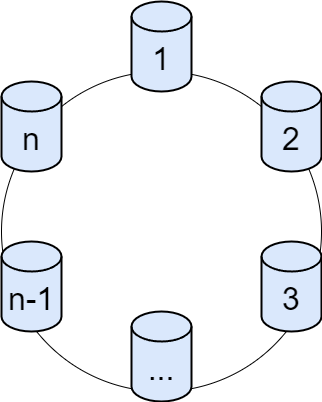
\includegraphics[width=2in]{Glass.png} 
        \caption{Glass in a circular arrangement}
       
    \end{minipage}%
    \begin{minipage}{0.5\textwidth}
        \centering
        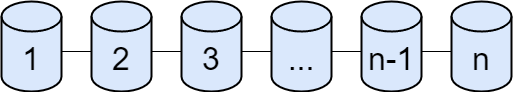
\includegraphics[width=\linewidth]{GlassLine.png} 
        \caption{Glass in a linear arrangement}
    \end{minipage}
\end{figure}

If one were \keyword{Clarification} to interpret `circular' as to `fill' in the space in the middle, then we can show that it is not optimal for Player A to put any liquid in that cup. This can be seen as a graph in graph theory. Each cup can be seen as a node on a graph and for example, we could have 6 glasses around a singular centre cup. Similar to Figure 1, but with an extra seventh cup in the middle. We set edges between nodes if they are touching and are adjacent to each other, giving Player B an opportunity to remove two adjacent nodes. If we count the degree of each node, then all cups on the outside would have degree three while the centre cup would have degree six. Why is this important? Because we are trying to prevent Player B from making us lose. Choosing cups with degree three gives Player B less choice of `hurting' our chances of winning. If Player A places any water in the middle cup, then there are now six different choices of adjacent cups to remove water as well. So we clarify the question to only have an arrangement similar to Figure 1. We explore an expansion of this game with middle glasses in our Review.

We will \keyword{I want} want to use what we stated to explore the following questions:
\begin{itemize}
    \item Who will win? Is someone always the victor?
    \item What is the winning strategy that they would use?
    \item Are there conditions for them win?
\end{itemize}

We define \keyword{Introduce} a \textit{winning strategy} as a sort of algorithm that can always lead to a win. A position can also be described as a \textit{winning position} if said position can ultimately end with a win, given a winning strategy is followed. On the other hand, a position can be described as a \textit{losing position} if no matter what action is done during a Player's turn, the opponent will end on a winning position. 

Moving on from these typical game theory definitions, we \keyword{Strategic Specialisation} attempt to solve games for $n=1$ and $n=2$. We can see that these are losing games for Player A and Player B always has a winning strategy of just to keep removing all the water from all the cups. Player A has no counter-strategy and thus would just forfeit.

\begin{figure}[h]
    \centering
    \begin{minipage}{0.5\textwidth}
        \centering
        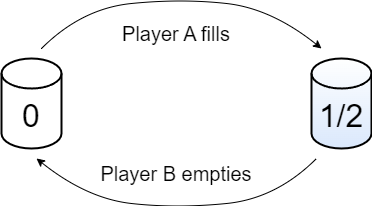
\includegraphics[width=2.7in]{1Glass.png} 
        \caption{$n=1$ Game}
       
    \end{minipage}%
    \begin{minipage}{0.5\textwidth}
        \centering
        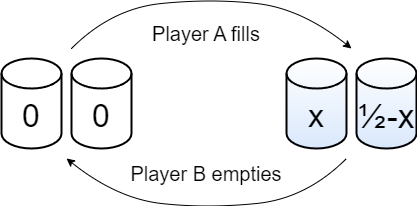
\includegraphics[width=3in]{2Glass.png} 
        \caption{$n=2$ Game}
    \end{minipage}
\end{figure}

These are trivial examples but give us a foundation to work from during our attack.


%--------------------------------------------------------------------------------------------------

\section{Attack} %---------------------------------------------------------------------------------


 We begin \keyword{Strategic Specialisation} our attack by exploring a game with $n=3$ glasses. Player A requires one glass to have greater than one pint of liquid. Receiving half a pint every turn, Player A needs a minimum of three turns before they can overfill a glass. Player B has a winning strategy that prevents any glass from being overfilled. Quite simply, they just rotate the pair of glasses that they empty and Player A has no winning moves. 

 Before formalising Player B's winning strategy, we write $(x, y)$ \keyword{Introduce} to refer to the pair of glasses labelled $x$ and $y$. We need these to be adjacent to each other otherwise Player B is making an illegal move. Now assuming the glasses are ordered 1, 2, and 3, Player B can empty the pairs $(1,2)$, $(2,3)$, and then $(3,1)$ continuously and this will stop any one glass from overfilling. As each glass has a maximum of one turn that it is not emptied, then no matter what Player A tries, they will not win and Player B wins! 
 
 \begin{table}[h]
     \centering
     \renewcommand{\arraystretch}{1.1}
     \begin{tabular}{|c|c|c|c|c|} \hline  
          Turn&  Action&  Glass 1&  Glass 2& Glass 3\\ \hline 
          1.A&  Fill all cups equally&  1/6&  1/6& 1/6\\ \hline 
          1.B&  Removes water from (1, 2)&  0&  0& 1/6\\ \hline 
          2.A&  Fill all cups equally&  1/6&  1/6& 2/6\\ \hline 
          2.B&  Removes water from (2, 3)&  1/6&  0& 0\\ \hline 
 3.A& Fill all cups equally& 2/6& 1/6&1/6\\ \hline 
 3.B& Removes water from (1, 3)& 0& 1/6&0\\ \hline
     \end{tabular}
     \caption{Game with $n=3$ glasses}
     \label{tab:my_label}
 \end{table}

Above we introduce \keyword{Introduce} a new method of representing on game, specifically in tabular form. We write turn $i$.A for Player A's $i^{th}$ turn and $j$.B for Player B's $j^{th}$ turn. We just chose Player A's strategy as filling all cups equally, however, even with other strategies, the closest we can get to winning is filling up a cup to exactly one pint (assuming we fill up one cup twice) before Player B removes all the water. Even with that strategy, Player B would have had to choose two empty cups to throw away before Player A is able to fill one cup.

We have seen that Player B always has a winning strategy for small values of $n$ so we may try \keyword{Try} a game with a larger amount of glasses. For large enough $n$, we conjecture \keyword{Conjecture} that Player A would only place water in every other glass and never next to a glass that already has water. 

To see that this is the \keyword{Justify} case, we can express a game of $n=8$ glasses as a graph as shown in Figure 5 below. Let our graph have weighted edges that hold the value of the sum of both adjacent nodes. Player A is best to play either only on the odd or even labelled nodes. Assume Player A chooses to play only on odd cups and has 0.2 pints of water in the odd glasses. Filling any water in even labelled nodes only gives Player B the advantage.

\begin{figure}[h]
    \centering
    \begin{minipage}{0.5\textwidth}
        \centering
        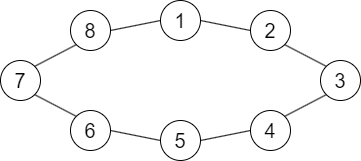
\includegraphics[width=2.6in]{Graph.png} 
        \caption{Graph of $n=8$ glasses}
       
    \end{minipage}%
    \begin{minipage}{0.5\textwidth}
        \centering
        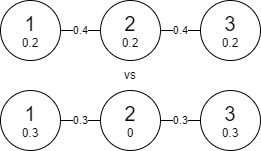
\includegraphics[width=2in]{justify.drawio.png} 
        \caption{Nodes 1, 2, and 3}
    \end{minipage}
\end{figure}

Say Player A fills \keyword{Justify} up cup 2 with 0.2 pints of water. Player B now gets the choice of removing pairs $(1,2)$ or $(2,3)$. By removing either pair, 0.4 pints of water is thrown away. If Player instead chose to split the water that would've gone into cup 2 into both cups 1 and 3, say equally, then those cups would have 0.3 pints. Then Player B can only remove a maximum of 0.3 pints, instead of the potential 0.4 pints before. In Figure 6, edges ${1,2}$ and ${2,3}$ have a value of 0.4 if even nodes are used whereas 0.3 if only using odd nodes. This highlights the fact that Player B's advantage is that they can only remove adjacent cups. Removing Player B's advantage is equal to playing a game with half as many glasses but Player B only removes one glass. If $n$ odd, then Player A should only play on $\frac{n-1}{2}$ isolated glasses and $\frac{n}{2}$ if $n$ even.

% maybe add picture

Even checking \keyword{Check} in our small case of $n=3$, Player A got closer to their goal by filling water into one isolated glass than spreading it out to adjacent glasses. Player A's general strategy may be to focus on certain isolated glasses in order to win. However, this wouldn't work as a strategy for Player A as Player B would always just remove the glass that Player A puts water in. \keyword{Stuck} If we were Player A, we would have to find a balance between filling up a few glasses while getting closer to our goal of filling up one glass.

In fact, let's see how Player A may win. Before Player A can win, there must be at least two separated glasses with more than 0.5 pints. This means that even if Player B removes one glass, there is another glass that Player A can overfill. \keyword{AHA} These glasses need to be strictly greater than 0.5 pints otherwise we would only completely fill up a glass before Player B removes the water again. As for Player B, a strategy would be to remove the pair of glasses with the largest value. This could be seen as the weighted edge with the largest value and choosing the adjacent glasses. However, if we assume that Player A only fills isolated glasses, then Player B would just pick the glass with the largest value and any glass on either side. We can \keyword{Try} try this example with $n=8$ and just observe what happens.

\begin{table}[h]
    \centering
    \begin{tabular}{|c|c|c|c|c|} \hline 
         &  \multicolumn{4}{|c|}{$i^{th}$ Pair of Glasses and Volume}\\ \hline 
         Turn&  1&  2&  3&  4\\ \hline 
         1.A
&  0.125&  0.125&  0.125&  0.125\\ \hline 
         1.B
&  $\times$&  &  &  \\ \hline 
         2.A
&  &  0.292&  0.292&  0.291\\ \hline 
         2.B
&  &  $\times$&  &  \\ \hline 
         3.A
&  &  &  0.542&  0.541\\ \hline 
         3.B
&  &  &  $\times$&  \\ \hline 
 4.A
& & & & 1.041\\ \hline 
 4.B
& & & & Lose\\ \hline
    \end{tabular}
    \caption{Split Strategy for game with $n=8$ glasses}
    \label{tab:my_label}
\end{table}

We simplify our table compared to Table 1 by combining glass pairs, so the first pair would be glasses $(1, 2)$ as in Figure 5 and vice versa. We also remove the `Action' column. We set our actions to be the same turn by turn; Player A splits the water (close enough to equally) to the active cups and Player B just throws away the cup with the highest volume. 

Now moving on to the result, this strategy for Player A seems to work well as they win and Player B is already playing optimally by removing the best pair of glasses. We can conjecture \keyword{Conjecture} that this strategy would work for any values of $n$ greater than 8. We will explore later what happens when $n < 4$.

We can see that this is \keyword{Justify} true by only observing the last column. Working backwards see that 0.5 pints is added on turn 4.A, 0.25 pints is added on turn 3.A, 0.166 pints is added on turn 2.A and we add 0.125 pints on turn 1.A. This is equal to the following sum.
\[
\sum^{k}_{i=1}{\frac{1}{2i}} \hspace{20pt} \text{s.t.} \hspace{20pt}  
k = \begin{cases} 
      \frac{n-1}{2} & \text{if $n$ odd}  \\
      \hspace{5pt} \frac{n}{2} & \text{if $n$ even}
   \end{cases}
\]

We have $k$ set to the \keyword{Justify} number of pairs. As stated above, there are $\frac{n-1}{2}$  isolated pairs of glasses if $n$ odd, and $\frac{n}{2}$ if $n$ even. Note that we will use \keyword{Introduce} $k$ as the number of pairs of glasses throughout the rest of the rubric. Also. note that our sum is the harmonic series multiplied by half, so knowing this, for any $n$ greater than 8, the final volume of water in the final glass will tend to infinity. This is much more than necessary as we only need it to be greater than 1 pint. We also know that if there are $k$ isolated pairs which in turn means that Player A will have at least $k$ turns before Player B can even remove all the water for each glass once. Thus this strategy is foolproof and we can even check that this is the case. 

We use this \keyword{Check}  strategy for greater values of $n$. With the help of Python, we find that this strategy indeed works for all values of $n \geq 8$. In the following table, we show what the final volume would be for $n \geq 6$ up to $n= 29$.  With our justification, we know that values above 29 will continue to work. However, from our table, $n=6$ and $n=7$ does not work. So we may have to either adjust our strategy or potentially conjecture that we need a minimum of $x$ amount of glasses for Player A to have a winning strategy. 

\begin{table}[h]
    \centering
    \renewcommand{\arraystretch}{1.1}
    \begin{tabular}{|c|c|c|c|c|c|c|c|} \hline 
         $n$&  Final Volume&  $n$&  Final Volume&  $n$&  Final Volume&  $n$& Final Volume\\ \hline 
         6
&  0.917
&  12
&  1.225
&  18
&  1.414
&  24
& 1.551
\\ \hline 
         7
&  0.917
&  13
&  1.225
&  19
&  1.414
&  25
& 1.551
\\ \hline 
         8
&  1.042
&  14
&  1.296
&  20
&  1.464
&  26
& 1.589
\\ \hline 
         9
&  1.042
&  15
&  1.296
&  21
&  1.464
&  27
& 1.589
\\ \hline 
 10
& 1.142
& 16
& 1.358
& 22
& 1.509
& 28
&1.625
\\ \hline 
 11
& 1.142
& 17
& 1.358
& 23
& 1.509
& 29
&1.625
\\ \hline
    \end{tabular}
    \caption{Final Volume after following Split Strategy}
    \label{tab:my_label}
\end{table}



%     \item Who will win? Does someone always win?
%     \item What is the winning strategy that they would use?
%     \item Are there conditions to them winning?
% mini re-entry
% min turns needed
% better strat
% least amount of glasses need

We pause to reassess our problem. \keyword{Mini Re-entry} After investigating our problem, we know that there are certain conditions for either player's win. For smaller values of $n$, Player B has a winning strategy, and for larger values of $n$, Player A has a winning strategy. We will continue to explore specifically what these conditions are by asking the \keyword{I want} following few questions:

\begin{itemize}
    \item Is there a better strategy for Player A?
    \item What is the least amount of $n$ glasses required for Player A to have a viable winning strategy?
    \item What is the minimum amount of turns needed for Player A to win?
\end{itemize}

It may seem that we are very much focused on Player A and to that I would agree. Player B's strategy is to prevent Player A from winning, so as long as Player A has a strategy that can counter Player B, they should win every time. Even if Player A were to make a mistake, they could always just continue the game in any state and follow our steps to win. Currently we have that Player A's Even Splitting Strategy for games of $n \geq 8$ is as follows: \\
\textbf{Step 1 -} Split water evenly among $k$ cups. Player B will then retaliate and remove one glass. \\
\textbf{Step 2 -} Split water evenly among the cups with water still left in them. Player B continues to repeat their move. \\
\textbf{Step 3 -} Repeat Step 2 until victory.

We notice that for very large games, \keyword{AHA} some glasses overflow before reaching the final glass. In fact, we can take this a step further to better refine Player A's splitting water strategy. As stated before, before Player A can win, at least two glasses need to have strictly greater than 0.5, so at any point, if there are glasses with more than 0.5 pints of water already in them, all Player A needs to do is to pour all their 0.5 pints into that glass and win. This is already a better strategy for Player A but we still don't know if we can win for games with $n=4,5,6,$ and 7 glasses. So we will want \keyword{I want} to now focus our attention on these last few games.

Knowing how we defined $k$, we will treat games of 4 and 5 glasses as one. They only have 2 isolated pairs of glasses. Similarly, games of 6 and 7 glasses are practically games with 3 isolated pairs of glasses. Beginning with the smaller of the two, we can quite easily show that Player B has a winning strategy. In a similar manner to our game with 3 glasses, all Player B has to do is alternate which pair of glasses they empty. If we order our glasses 1, 2, 3, and 4. Throwing away the pairs (1, 2) and $(3, 4)$ every other turn will result in victory. 

Acting as Player A, we attempt a strategy of replacing what was thrown away and splitting the rest. \\
\textbf{Step 1 -} Split water evenly among 2 isolated cups.\\
Player B will remove water from one glass as they are indifferent.  \\
\textbf{Step 2 -} Replace the water lost and continue to split the leftover water evenly. \\
Again Player B repeats their action. \\
\textbf{Step 3 -} Repeat Step 2. \\

\begin{table}[h]
    \centering
    \renewcommand{\arraystretch}{1.3}
    \begin{tabular}{|c|c|c|c|c|c|c|c|c|c|} \hline  
 & \multicolumn{9}{|c|}{Player A's $i^{th}$ turn}\\ \hline  
         &  1&  2&  3&  4&  5&  6&  7&  8& 9 \\ \hline  
         Volume&  0.25
&  0.375
&  0.4375
&  0.46875
&  0.48438
&  0.49219
&  0.49609
&  0.49805
&  0.49902
\\ \hline  
 & $\frac{ 1 }{ 4 }$
& $\frac{ 3 }{ 8 }$
& $\frac{ 7 }{ 16 }$
& $\frac{ 15 }{ 32 }$
& $\frac{ 31 }{ 64 }$
& $\frac{ 63 }{ 128 }$
& $\frac{ 127 }{ 256 }$
& $\frac{ 255 }{ 512 }$
& $\frac{ 511 }{ 1024 }$
\\ \hline  
 Leftover& 
0.25
& 0.125
& 0.0625
& 0.03125
& 0.01562
& 0.00781
& 0.00391
& 0.00195
& 0.00098
\\ \hline  
 & $\frac{ 1 }{ 4 }$ & $\frac{ 1 }{ 8 }$ & $\frac{ 1 }{ 16 }$ & $\frac{ 1 }{ 32 }$ & $\frac{ 1 }{ 64 }$ 
& $\frac{ 1 }{ 128 }$ & $\frac{ 1 }{ 256 }$ 
& $\frac{ 1 }{ 512 }$ 
& $\frac{ 1 }{ 1024 }$ \\ \hline 
    \end{tabular}
    \caption{Replace and Split Strategy for game $n=4$}
    \label{tab:my_label}
\end{table}

We get the following results. This can be turned into a conjecture: \keyword{Conjecture} the best or closest to winning that Player A can achieve in a game with 4 glasses is reaching 0.5 in two cups. To show that this is the case, we highlight the bottom row is equal to the following sum.
\[
\sum^{i}_{j=1}{\frac{1}{2^{j+1}}} \to 0.5 \hspace{10pt} \text{as} \hspace{10pt} i \to \infty
\]
This sum \keyword{Justify}shows that 0.5 pints is the maximum amount of water in either cup if Player A plays for infinite turns. As it takes two turns for Player B to `clear' all water, this is the maximum achievable volume. This is given that Player B plays optimally because technically if Player B follows a set pattern, Player A could fill one pair twice getting 1 pint but that requires Player B to choose to throw away empty cups. We stated something similar in the case of $n=3$.

Even still, Player A will not meet the conditions of having 2 glasses of over 0.5 pints. Therefore games of $n \leq 5$ glasses will be losing games \keyword{AHA}for Player A and winning for Player B. Hopefully we can use what we've learnt here to adapt our strategy for the $n=6$ and 7 case. With that being said, we move to such cases. With $k = 3$ we go back to our splitting strategy to see what went wrong. \keyword{Stuck} We get the following table. 


\begin{table}[h]
    \centering
    \begin{tabular}{|c|c|c|c|} \hline 
         &  \multicolumn{3}{|c|}{$i^{th}$ Pair of Glasses and Volume}\\ \hline 
         Turn
&   1&2& 3\\ \hline 
         1.A
&   0.167&0.167& 0.166\\ \hline 
         
1.B
&   $\times$&& \\ \hline 
         2.A
&   &0.417& 0.416\\ \hline 
 2.B
&  &$\times$&\\ \hline 
 3.A
&  &&0.917\\ \hline 
 3.B
&  &&$\times$\\ \hline
    \end{tabular}
    \caption{Split Strategy on Game with $n = 6$ or 7 glasses}
    \label{tab:my_label}
\end{table}

We see that on turn 2.A we do \keyword{AHA} not have two glasses with over half a pint. We add 0.25 pints to pair 2 and 3 when they have 0.167 (or 0.166) from turn 1.A. However, Player A wants these to be at least half a pint. One should then only add 0.25 pints only when these cups have at least 0.25 pints. This iterative process can be seen below in Figure 7. Visually we can see that, as stated before, we need at least two cups with more than half a pint, but now we can also see that the step before that Player A will need at least three glasses with more than a quarter pint. This can be seen as a winning position. As long as Player A has a strategy to get to this position, they can always win. In fact, this could have been done for our simple Even Splitting Strategy. As long as we have three cups with more than a quarter pint, our steps can end early and we can just play as shown below. The issue \keyword{Stuck} is how do we get to the point that we have this situation. We have seen above that simply splitting our glasses evenly fails.  \\
\\

\begin{figure}[h]
   \centering
   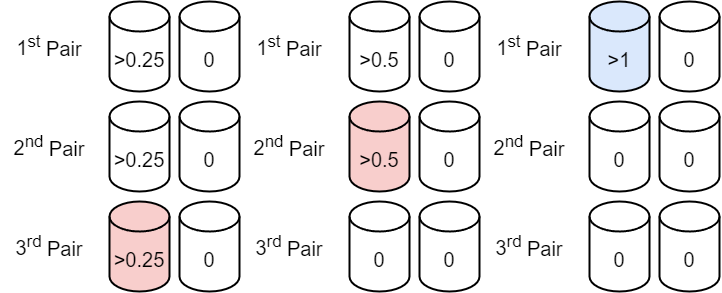
\includegraphics[width=4in]{3CupStrat.png}
   \label{myfig}
   \caption{Necessary Condition for Player A's Win}
\end{figure}

We try and \keyword{Try} employ a mixed strategy of our two previous strategies. We follow the iterative process: \\
\textbf{Step 1 -} Split the liquid evenly across three glasses. \\
Player B then removes one of the cups \\
\textbf{Step 2 -} We replace the lost liquid in the now empty cup and split the remaining liquid evenly  \\
Again, Player B then removes one of the cups as they are all the same \\
\textbf{Step 3 -} Split the water evenly between the two glasses with water in them\\
Player B removes one of the two cups with water \\
\textbf{Step 4 -} Pour all the water into the final glass with water still left in it\\
Player A has won! \\
We can check that this \keyword{Check} strategy works in the following table.
\begin{table}[h]
    \centering
    \renewcommand{\arraystretch}{1.3}
    \begin{tabular}{|c|c|c|c|c|c|l|l|} \hline 
 & \multicolumn{7}{|c|}{Turn}\\ \hline 
         &  1.A&  1.B&  2.A&  2.B& 3.A& 3.B& 4.A\\ \hline 
         Pair 1&  $\frac{1}{6}$&  &  $\frac{5}{18}$&  &  $\frac{19}{36}$& & $\frac{37}{36}$\\ \hline 
         Pair 2&  $\frac{1}{6}$&  &  $\frac{5}{18}$&  &  $\frac{19}{36}$& $\times$& \\ \hline 
         Pair 3&  $\frac{1}{6}$&  $\times$&  $\frac{5}{18}$&  $\times$&  & & \\ \hline
    \end{tabular}
    \caption{Winning Strategy}
    \label{tab:my_label}
\end{table}

Thus we have a Winning Strategy for Player A. On turn 1.A, we apply Step 1, splitting the half pint evenly among the three pairs of cups. As there is no difference in choice for Player B, they would just remove whichever pair they want, in this case, we said Pair 3. On turn 2.A, Player A applies Step 2 and replaces the 1/6 that was lost. They take the remaining $1/2 - 1/6 = 1/3$ \keyword{Check} pints of liquid and split it evenly into the three pairs. This gives us the $1/6 + 1/9 = 5/18$ pints and as $\frac{5}{18} > 0.25$, Player A can follow what is shown in Figure 7. On 2.B, Player B removes an indifferent pair, say Pair 3. Following Step 3, Player A creates two glasses with $5/18 + 1/4 = 19/36$ pints of water. Player B responds by removing one of the two pairs and Player A wins by pouring all their half pint of water into the final glass. Victory! \keyword{AHA}

We still have one last question to answer: \keyword{Stuck} `What is the minimum amount of turns needed for Player A to win?'. We answer with the following conjecture; \keyword{Conjecture} the fastest Player A can win for a game with more than six glasses is for Player A to play four turns. This is under our assumption of rational play. We know that \keyword{Justify} Player A needs at least three turns before they can ever have more than one pint of water in one glass. Thus after Player A has 3 turns, a maximum of 1.5 pints of liquid could be on the board at any one time (assuming that no liquid is thrown away). However, we know that Player B will always have a chance to remove some amount of water. This is shown in Table 6. Assume that we didn't split our water evenly, then there would be at least one cup with a value greater than $1/6$. This would then be targeted as it is a dominant target. We take dominant target \keyword{Introduce} to mean that any other strategy is sub-optimal, thus Player B, playing rationally, would remove the said cup. So $1/6$ is the minimum amount of water that Player B would get rid of in turn 1.B. 

We move to turn 2.A under \keyword{Justify} the assumption that Player B removed the minimum of $1/6$ pints of water. There is currently $1/3$ of a pint of water in the glasses. Then we can apply the same logic that if we don't evenly split the liquid, there will be a dominant target. Thus a minimum of $1/6 + 5/18 = 4/9$ pints of liquid will be removed from the game if Player B plays optimally. The leftover $1.5 - 4/9 = 19/18$ pints of water will be split between two cups. Which implies a win on turn 3.A is impossible. Therefore, knowing our Winning Strategy works for any game with more than six glasses and wins in 4 turns, this is indeed the minimum amount of turns needed for Player A to win.

%--------------------------------------------------------------------------------------------------

\section{Review} %---------------------------------------------------------------------------------

    % \item Who will win? Is someone always the victor?
    % \item What is the winning strategy that they would use?
    % \item Are there conditions to them winning?
    %  \item Is there a better strategy for Player A?
    % \item What is the least amount of $n$ glasses required for Player A to have a viable winning strategy?
    % \item What is the minimum amount of turns needed for Player A to win?

Reviewing our initial questions, \keyword{Check} we found that victory is conditional on $n$, the number of glasses. For $n < 6$, Player B can always win and for $n \geq 6$, Player A can always win following the strategy we described above. namely the `Winning Strategy'. In fact, we found that the `Winning Strategy' is the fastest strategy for Player A to win. 

Overall, \keyword{Reflect} we have done what we set out to accomplish, answering our initial and second set of questions. I am quite happy with the results that we managed to achieve. By answering these questions, we have `solved' the game. A solved game is a game in which the outcome can be determined from any position, with the assumption that players are acting rationally. I take this to be the greatest achievement that I am most proud of. This relates quite well to the Matrix game from Assignment 2 where if the player using 1 were to go first, they could only win for small sized matrices. In that rubric, I reflected on the power of a few well placed zeros, but in this problem, a few small sums can easily negate any amount of reduction to it.

There \keyword{Reflect} were a couple of challenging parts. Initially, I found it a bit difficult to explain certain ideas, however, with hindsight, I should have immediately utilised visual aids in the form of pictures and tables. I consistently refer to these figures and tables throughout and help organise data much more clearly. Before, I would spend more effort writing long paragraphs that were not clear or concise. I also thought that my lack of graph theory knowledge would make it difficult to describe our game. Luckily enough, I went down a different route of expressing our game that didn't require more in-depth knowledge of that field. We were able to simplify our game so that only basic graphs were needed. I'm sure with greater knowledge of graph theory, we could relate it to a grander picture but alas, that is not where my specialty lies.

Besides \keyword{Reflect} some initial setbacks, Python was always extremely helpful. Whether it be quickly calculating our strategies, checking for various cases, or even helping print LaTeX code, Python was great at uncovering certain behaviours. For example, by methodically checking each iteration of our initial splitting strategy, we managed to find ways of optimising it. 

Throughout the \keyword{Reflect} rubric I have learnt of a couple of approaches that would help with making my arguments clearer. If I were to redo my entire rubric, I may have dropped the terms Player A and Player B. Initially I thought that using Player A and B was better but writing Ali and Beth is in fact more differentiable. Another point of clarity would be to immediately state that we would act as Player A. Through the perspective of Player A, we would be more easily differentiated from Player B, our opponent. There were a few times where I would write `we', already acting as Player A, instead of writing `Player A'. I stated why this is the case in the middle of the attack; Player B has a very set strategy of preventing Player A from winning, thus we only need to focus on what changes Player A would make to win. 

Other than imperfect\keyword{Reflect} writing with perspective issues, another issue I could have addressed more clearly is that Player B is assumed to just remove the water from the pair of glasses with the largest total volume. After we explained that Player A would only play in isolated cups, I should have made it certain that Player B had no other strategy than to choose the glass with the largest volume. We did explain it thoroughly but only quite deep into our attack. There is always room for improvement and will be a good lesson for later in my problem solving journey.

We have already stated some ways to \keyword{Extend} extend the game. From our Entry, we said even if the middle were full of glasses, there would be no benefit for Player A to place water there. In fact, it is detrimental to their strategy. However, say we give another condition to Player A's win and that they must always add some amount of water to a cup in the middle. Let's say at least 0.1 pints. We may then have the following strategy.

\begin{figure}[h]
   \centering
   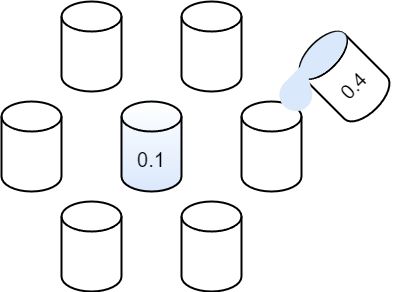
\includegraphics[width=2in]{NewGame.png}
   \label{myfig}
   \caption{New Potential Game}
\end{figure}
We, acting as Player A now, just `sacrifice' 0.1 pints of water \keyword{Try} every round and see what comes of it. We get the following table. 
\begin{table}[h]
    \centering
    \renewcommand{\arraystretch}{1.3}
    \begin{tabular}{|c|c|c|c|c|} \hline 
 & \multicolumn{4}{|c|}{Glasses and Volume}\\ \hline 
         &  Middle&  Pair (1, 2)&  Pair (3, 4)&  Pair (5, 6)\\ \hline 
         1.A
&  $\frac{1}{10}$&  $\frac{2}{15}$&  $\frac{2}{15}$&  $\frac{2}{15}$\\ \hline 
         1.B
&  $\times$&  $\times$&  &  \\ \hline 
         2.A
&  $\frac{1}{10}$&  $\frac{ 2 }{ 9 }$&  $\frac{ 2 }{ 9 }$&  $\frac{ 2 }{ 9 }$\\ \hline 
         2.B
&  $\times$&  $\times$&  &  \\ \hline 
 3.A
& $\frac{1}{10}$& $\frac{ 38 }{ 135 }$& $\frac{ 38 }{ 135 }$&$\frac{ 38 }{ 135 }$\\ \hline 
 3.B
& $\times$& $\times$& &\\ \hline 
 4.A
& $\frac{1}{10}$& $\frac{ 26 }{ 81 }$& $\frac{ 26 }{ 81 }$&$\frac{ 26 }{ 81 }$\\ \hline 
 4.B& $\times$& $\times$& &\\ \hline
    \end{tabular}
    \caption{New Game Strategy}
    \label{tab:my_label}
\end{table}
Similarly to our Winning Strategy, we now instead have 0.4 pints to distribute to our three outer pairs of glasses. 0.1 pints of water is being used to fulfil our new condition. We employ the strategy of replacing the lost liquid and splitting the rest. If we start from the beginning, $0.4/3 = 2/15$. When our second turn comes, we now only have $(0.4 - 2/15)/3=4/15$ pints left to split, so each pair is now $2/15 + 4/45=2/9$.  After following this pattern we find that even though $38/135$ is greater than 0.25 but we actually need \keyword{Stuck} to continue further before we can switch to having something similar to that of Figure 7, our win condition. This is because we now only have 0.4 pints of distributable water, therefore in order to have one cup overflow, the previous turn we would need two cups to have at least 0.6 pints of water. The turn before that we would need three cups to have $7/15$ pints of water. With Python, we find that our strategy can only get us a maximum of 0.4 pints in three cups. Thus, we have a losing game. \keyword{AHA} We find the volume of water of any pair on turn $i$ follows

\[
a_i = a_{i-1} + \frac{0.4 - a_{i-1}}{3} \hspace{10pt} \text{and} \hspace{10pt} a_0 = \frac{0.4}{3}
\]

This may be useful for our later extension. On \keyword{Check} Python, we check that this indeed follows what we have in our table.

Before moving any further, here are some similar and not so similar ideas of how to \keyword{Extend} extend our game and even further questions to ask:
\begin{itemize}
    \item What if we have $x$ pints of water to distribute over $n$ glasses.
    \begin{itemize}
        \item What would be the minimum amount of $x$ for us to still win?
    \end{itemize}
    \item What if we need to have two glasses to overflow? 
    \item We could combine the two points above to have our game be:  We need $y$ glasses to overflow with $x$ pints to distribute.
    \item What if the glasses can hold $y$ pints of liquid.
    \item Could we add another player? A  new Player C with a different liquid, say oil, so that it floats over the water. They win by spilling oil before Player A can win.
\end{itemize}

To \keyword{Extend} address the first point, we have something similar to our new potential game as shown in Figure 8, if we set $n=3$. In that game, we practically lost 0.1 pints to the middle cup, however, we found that we weren't able to fill any one cup over 1 pint. That does give us a good baseline to work with as we'll need to find the value $0.4 < x < 0.5$ such that we, Player A, can still win. We \keyword{Try} will still try to use our strategy of replacing lost liquid and splitting evenly. This method forces Player B to remove the least amount of water and consistently allows us to have $x$ pints of liquid in all three cups. Before attempting to solve this question, we have the following generalisation of Figure 7 explaining the winning condition for a game with $x$ pints of water that we distribute.

\begin{figure}[h]
   \centering
   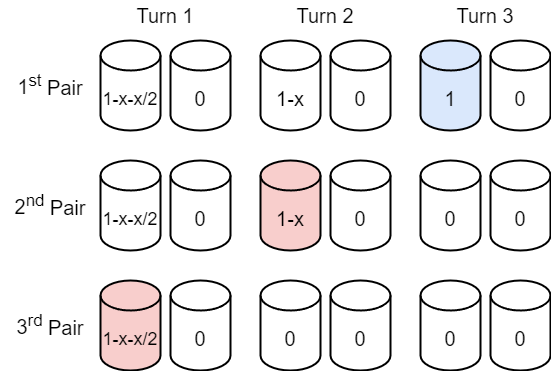
\includegraphics[width=3in]{WinCon.png}
   \label{myfig}
   \caption{Generalised Win Condition}
\end{figure}

This picture shows the end of each turn and how if we have three glasses with at least $1-x-x/2$ pints of water, we can win. As explained with $x=0.5$, if we want to have one final glass with over a pint of water, we need to fill two glasses up to $1-x$ pints before Player B removes one of these glasses. If we go back one more step, to get two glasses to have $1-x$ pints, we will need to fill up three glasses to have at least $1-x-x/2$ pints of water so when Player B throws away one, we have two glasses of $1-x-x/2$ pints to fill up with our $x$ pints of water. \keyword{AHA} f we put in $x=0.4$ from our previous extension we find that we cannot achieve this as $1-x-x/2=0.4$ which is just over what we could potentially produce with our replace and split strategy after playing infinite turns. Therefore, to answer our question, we only need $0.4+\varepsilon$ pints of water to distribute where $\varepsilon>0$. \keyword{Check} Testing this out in Python, we find that even for $x=0.40001$ pints of water, if we use our sum for $a_i$ with $a_0=x/3$, we get a value of $a_i>0.4$ for $i=31$. From Figure 9, we find that $1-x-x/2=0.3999\dots$ and as $a_{31}>0.4$ we can let Player B remove one of our three pairs. We then split our $x$ into the two remaining glasses so our first and second pair has $>0.6$ pints. After Player B removes one of the two glasses, we win by pouring all our water into the last glass. \keyword{Clarification} We only need $a_i>1-x-x/2$ as that is the only condition to have more than enough water to overfill the glass.

Of course \keyword{Assumption} this assumes that everything in the world is ideal and that we can perfectly split water down to the atomic level. Even still, we have an answer to the minimum amount of water needed to split over 6 glasses is $x>0.4$. We can now move away from our specific parameters \keyword{Extension} and choose other $x$ and $n$. Firstly, we test our \keyword{Try} current replace and split strategy for different values of $n$ in Python and find that it always generates isolated glasses with less than $x$ amounts of liquid. We can \keyword{Justify} understand why by realising that Player B can only remove at most $x$ liquid if we keep splitting our $x$ evenly throughout our turns. Thus, even though one cup is constantly being removed, all the rest of the cups can keep increasing up to the limit $x$. This gives a good baseline to work from. We can even further generalise \keyword{AHA} Figure 9 to have $k$ isolated pairs. If we have four pairs we can go back a turn and show that we only need to reach a minimum of four glasses having at least $1-x-x/2-x/3$ pints of liquid before we can win. So our mixed strategy of reaching our win condition with through the replace and split strategy seems to work extremely well for general games. We saw that more glasses always help us as Table 3 shows how even just splitting without replacing can generate many overflowing glasses.

With \keyword{Reflect} all that's been said, this rubric has been a fun and rewarding process. Exploring different aspects of this game has made us delve into topics of graph theory, harmonic series, and game theory. From such a simple idea of a game to reaching various fields of mathematics. Truly highlights the expanse of maths and how so many areas can be used in problem solving, even for seemingly trivial games. 

\section*{Supplementary material}
The code for this assignment can be found on my GitHub page:  \url{https://github.com/LazyTim/MA3K7/blob/main/MA3K7%20-%20Big%20Mini%20Project.ipynb}.



\end{document}
